\chapter{TnT UI}
\label{ch:ui}

TnT UI (Touch and Test User Interface) provides a graphical interface for doing following things:

\begin{itemize}
	\item Move the robot
	\item Control camera and view camera image
	\item Calibrate the system
	\item Position tips and DUTs
	\item Position physical buttons
	\item Run Touch Panel Performance Test scripts (if TPPT feature is included)
	\item Create test sequences (if Sequence Generator is included)
	\item Teach icons (if HSUF is included)
	\item Perform User Interface Performance measurements with High speed camera. (if HSUP feature is included)
\end{itemize}

In addition to this user manual, UI also has separate helps embedded in the different views and tooltips in use. The helps can be opened by clicking the white question mark inside a blue circle and tooltip texts appear automatically as tips are hovered on top of the input field. 

\section{Installing/re-installing TnT UI}
\label{sec:ui_installation}
Installation can be done by running the installation package. It launches a wizard that will help the user through the installation process. To run the UI a dedicated HASP USB encryption dongle has to be connected to the measurement PC. 

\subsection{Windows}
A valid license text file has to be available with the following path: "\tntLicensePath".

In case the user wants to re-install the UI, the following procedure should be followed in order to keep the configuration unchanged:
\begin{enumerate}
	\item \label{itm:ui_first} Go to the folder "\tntRootPath"  and create a back-up of existing "\tntUIFolder" folder by renaming the folder as "TnT UI 2020-01-02" where the date is the backup date.
	\item Run installation package as usual (the installer will create a new "\tntUIFolder" folder)
	\item Go to the old folder that you renamed in step \ref{itm:ui_first} and there to the "configuration". In that folder you should have "logging.yaml" and "start.yaml". Copy those and replace the files in respective folder created during installation.
\end{enumerate}

\subsection{Macos}

A valid license text file has to be available with the following path: "\tntLicensePathMacos".

The installer is a shell script with embedded data and can be ran from command-line. Once executed, the installer will prompt user to continue installing the package.
%
\begin{enumerate}
	\item Run the installation script from any location. The installer will create a backup of existing installation and copy new files under "\tntRootPathMacos\tntUIFolder". 
	\item The configuration directory is automatically copied from the latest backup to the new location by the installer.
\end{enumerate}

\section{Starting up}

\begin{figure}[h]
	\centering
	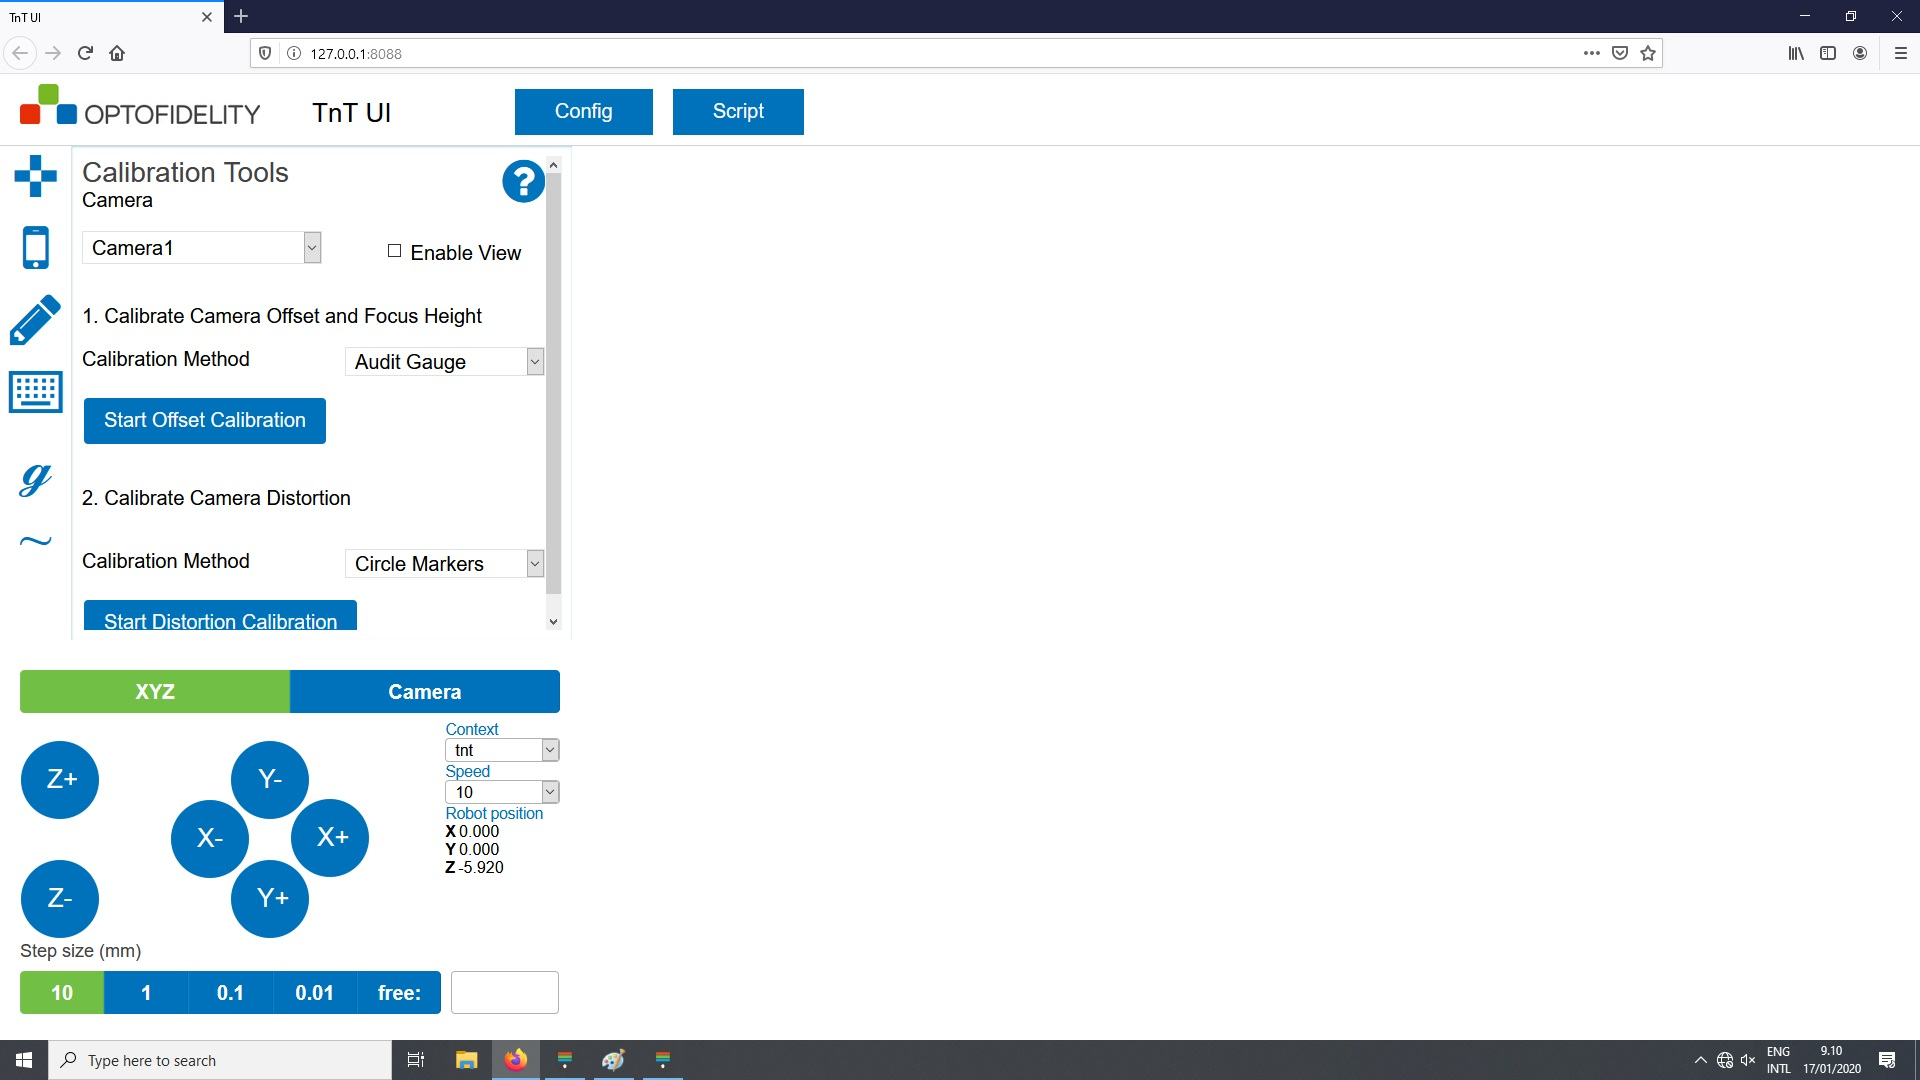
\includegraphics[width=0.7\linewidth]{ui_start.jpg}
	\caption{PC after successful UI initialization.}
	\label{fig:ui_start}
\end{figure}

Before starting UI, please make sure that the server has successfully been started. The UI can be started by double clicking the icon on the desktop. It is also possible to run the "\tntUIExecutable" directly. It can be found from the folder "\tntRootPath\tntUIFolder". It should first initialize a new terminal window and then open web browser (if not yet open) and show UI in address http://127.0.0.1:8088/. Please refer to Figure \ref{fig:ui_start} to see how PC should look like after successful UI initialization.

\section{Camera calibration}

\begin{figure}[h]
	\centering
	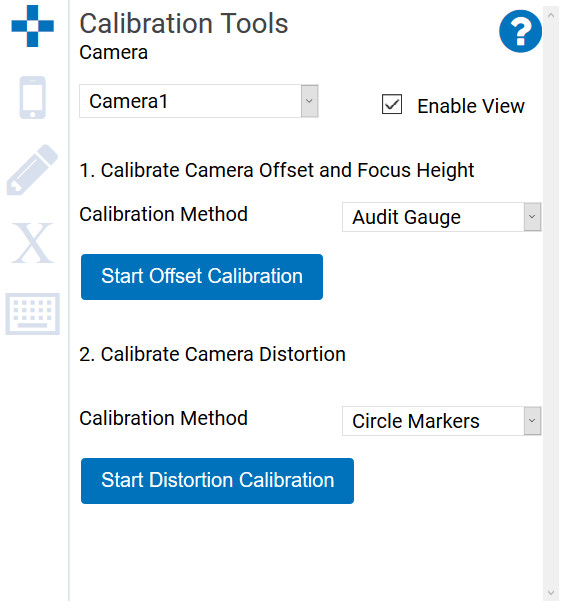
\includegraphics[width=0.4\linewidth]{ui_camera_calib.jpg}
	\caption{Camera calibration view in TnT UI.}
	\label{fig:ui_camera_calib}
\end{figure}

TnT UI Config page has a view for camera calibrations as shown in Figure \ref{fig:ui_camera_calib}. These must be performed before camera can be used in any actual operations such as moving robot from camera image, positioning DUTs using camera or performing functional testing.

Camera calibrations are done during delivery bring up by Optofidelity engineers. User may need to repeat the calibrations in case anything related to camera changes. This could be change in camera focus distance or change of camera objective.

\input{from_ui_repo/camera}


\section{Position DUTs}

This section contains instructions for positioning DUTs with the TnT UI. The UI Configs page has DUTs view for DUT positioning as shown in Figure \ref{fig:ui_duts}.

\begin{figure}[h]
	\centering
	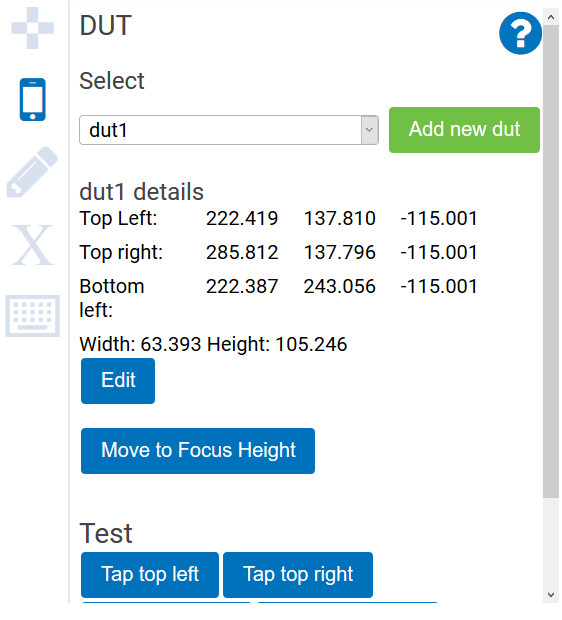
\includegraphics[width=0.4\linewidth]{ui_duts.jpg}
	\caption{DUT positioning view in TnT UI.}
	\label{fig:ui_duts}
\end{figure}

\input{from_ui_repo/duts}
 
\section{SVG shapes for a DUT}
For non rectangular DUTs the TnT software suite offers a possibility to define the shape as an SVG image. The SVG can be created using any suitable software, for example Inkscape. The SVG is added in the DUT edit pane and which stores it in "\svgFilePath".

A rough guide to SVG drawing with Inkscape can be found from Appendix \ref{app:inkscape_guide}.

\subsection{SVG shape requirements}
\label{sec:svg_shape_requirements}
In the SVG file, two regions need to be defined as paths:
\begin{enumerate}
	\item \texttt{analysis\_region}: This is the region to be tested.
	\item \texttt{bounding\_box}: This is the smallest rectangle that contains the whole analysis\_region. 
\end{enumerate}

It is important that both two regions are named exactly as above and that both of them are paths (not, for example, rectangles or circles). Also, both paths need to belong into same group, the name of the group does not matter. The size of the regions must be the same as the DUT size. Please see figure \ref{fig:svg_example} for reference. 

\begin{figure}[h]
	\centering
	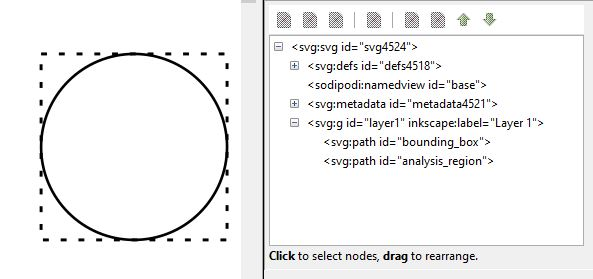
\includegraphics[width=0.7\linewidth]{svg_example.jpg}
	\caption{Example of SVG shape for a round DUT in Inkscape. The solid line shows the analysis\_region and the dashed line the bounding\_box.}
	\label{fig:svg_example}
\end{figure}

\warningbox{If the size of SVG shape does not match with actual DUT size, the TPPT test patterns might be missing lines and points in the edge areas.}

\subsection{The usage of SVG shapes}
The main usage of SVG shapes is to filter lines and points in TPPT scripts so that the robot does not try to touch areas outside the non-rectangular DUTs. Please see Figure \ref{fig:patterns_svg_filtered} for reference.  You can find example SVG (EmulatorRound.svg) from server resources folder in the server installation.

\begin{figure}[h]
	\centering
	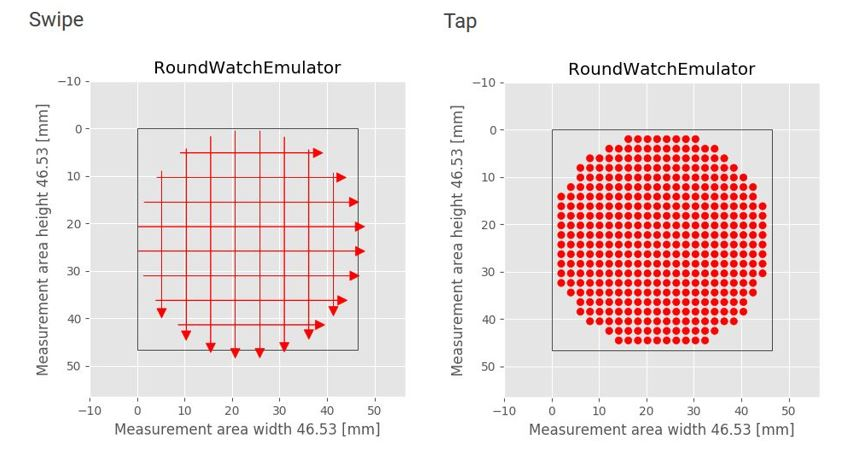
\includegraphics[width=0.7\linewidth]{patterns_svg_filtered.jpg}
	\caption{Examples of swipe and tap test grids for a round DUT}
	\label{fig:patterns_svg_filtered}
\end{figure}

In addition, the positioning image in the automatic DUT positioning is affected by SVG shapes and the image looks different depending on whether the DUT has an SVG shape defined or not. If there is no SVG defined for the DUT, the algorithm uses generic parameters for drawing the positioning image (such as ppmm). If the SVG shape is defined, the algorithm can calculate the exact parameters. However, for most cases, the automatic positioning works similarly with and without an SVG image.

\section{Tips}

\begin{figure}[h]
	\centering
	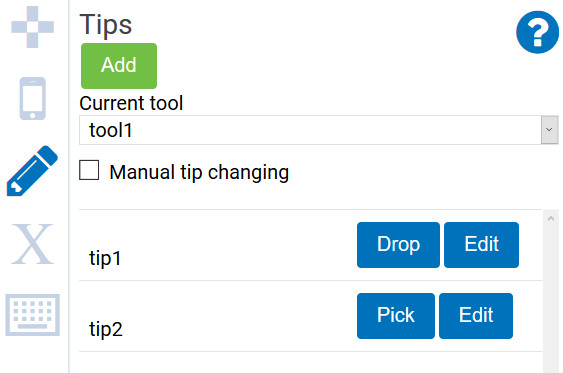
\includegraphics[width=0.4\linewidth]{ui_tips.jpg}
	\caption{Tips view in TnT UI.}
	\label{fig:ui_tips}
\end{figure}

Tip can be added, deleted and attached/detached to robot from TnT UI Config page in Tips view as shown in Figure \ref{fig:ui_tips}.

\input{from_ui_repo/tips}

\section{Icon teaching}
\label{sec:ui_icon_teaching}

\begin{figure}[!h]
	\centering
	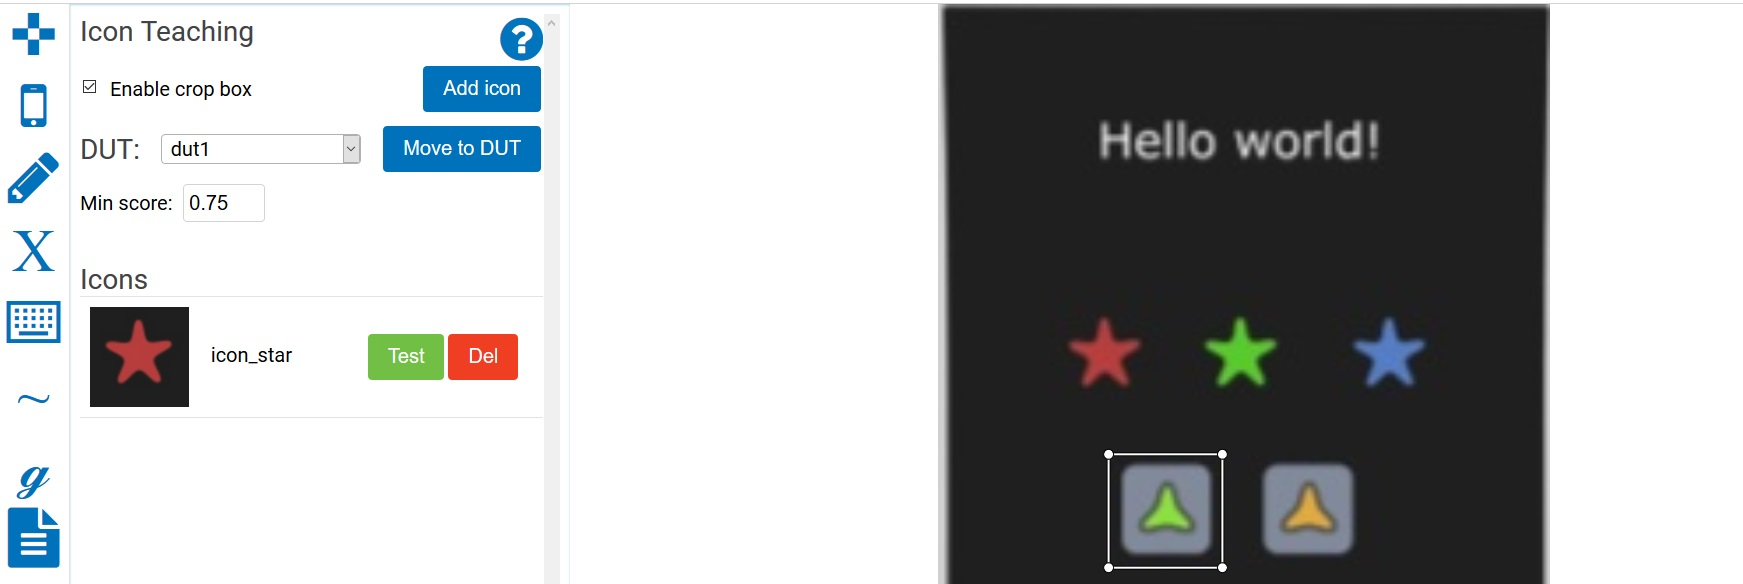
\includegraphics[width=\linewidth]{ui_icon_teaching.jpg}
	\caption{Icon teaching view in TnT UI. On the left side user can create, delete and test icons. On the right user can see the DUT in camera view and adjust crop box to define new icons.}
	\label{fig:ui_icon_teaching}
\end{figure}

TnT UI has "Icon teaching" view under "Config" page where user can teach icon models by using camera view and a crop box. This is shown in Figure \ref{fig:ui_icon_teaching}. The cropped image and icon shape model are stored in TnT Server under \texttt{data/icons} directory so that they can be later used via TnT Client to build functional testing scripts. Icons can also be created from image data in Python scripts using TnT Client.

\input{from_ui_repo/icon_teaching.tex}

\section{Physical buttons}

Physical buttons can be added, deleted and tested in TnT UI config page in Physical buttons view.

\input{from_ui_repo/phys_button}

\section{Force calibration}
\label{sec:force_calibration}

TnT UI Config page has Force calibration view as shown in Figure \ref{fig:ui_force_calib} to calibrate voicecoil based force actuator.

\begin{figure}[h]
	\centering
	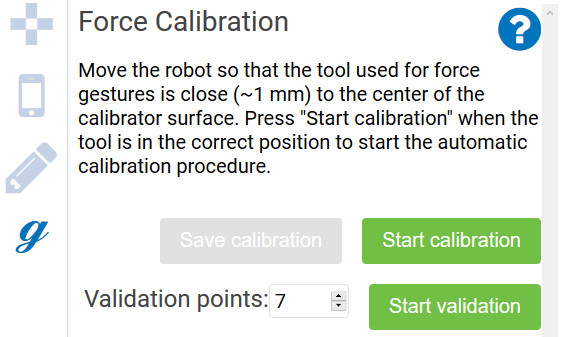
\includegraphics[width=0.4\linewidth]{ui_force_calib.jpg}
	\caption{Force calibration view in TnT UI.}
	\label{fig:ui_force_calib}
\end{figure}

\input{from_ui_repo/force_voice_coil}

\input{from_ui_repo/force_closed_loop}

\section{IO}

TnT UI Config page has IO (Input and Output) view as shown in Figure \ref{fig:ui_io}.

\begin{figure}[h]
	\centering
	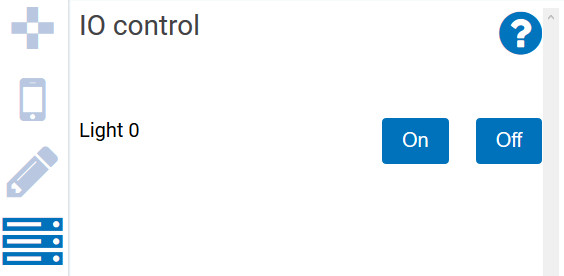
\includegraphics[width=0.4\linewidth]{ui_io.jpg}
	\caption{IO view in TnT UI.}
	\label{fig:ui_io}
\end{figure}

\input{from_ui_repo/io}

\section{Sequence generator}

\input{from_ui_repo/sequence_generator}

\section{UI troubleshooting}
In this section we have collected the most common issues encountered by our customers. In case you cannot find solution from here, please contact OptoFidelity support. More information about support can be found from Part \ref{part:support}.

\subsection{Common notes}
Many of the issues that are found when using UI are originating from server. The following list will provide you with links to the server troubleshooting:
\begin{itemize}
	\item Robot not moving, please refer to Section \ref{subsec:robot_not_moving}
	\item Camera image not shown, please refer to Section \ref{subsec:camera_issues}
\end{itemize}

\subsection{Camera distortion calibration fails}
 This can be caused by various reasons. Ensure that the entire chess pattern target is visible in the camera view. Adjust the exposure and/or gain until the image is clear, sharp, and with good contrast. The chess pattern should be plain black and white, without shades or reflections. It might be necessary to adjust the room lighting or use something to shadow the reflections away.

\subsection{Audit gauge lit inlet is not found automatically}
The reason for this is usually in camera settings or lighting conditions. Try to adjust camera exposure and/or switch off lights in the room.

\subsection{Automatic DUT positioning: cannot find blobs}
The reason for this is usually in camera settings or lighting conditions. Try to adjust camera exposure and/or switch off lights in the room. Also the brightness of the DUT screen might affect. 

\subsection{Automatic DUT positioning: cannot connect to DUT}
Please check the following things and try to go back to another view and then come back. A successful DUT connection is also shown in server terminal log messages (please note that the DUT name in log differs from the one you have given):
\begin{itemize}
	\item Check that the DUT is connected to the correct WiFi network.
	\item Check that the IP address is correct in the DUT app.
	\item Check that the DUT name is the same in the UI and DUT app.
\end{itemize}

\subsection{Adding SVG: The SVG dimensions do not match the DUT dimensions}
First check that the SVG is drawn correctly. If you have used Inkscape for drawing the DUT, please check also that the dimensions are shown as geometrical dimensions and not as visual dimensions. This can be done by going to "Edit"->"Preferences"->"Tools" and making sure that the "Geometric bounding box" is selected.
